\chapter{Data} 
\label{2.Data}
\lhead{\emph{Data}}

% https://www.datacamp.com/community/tutorials/matplotlib-3d-volumetric-data


% Todo empieza con MICCAI2008
% Explota con MICCAI2016

% TODO: Improve
The two main datasets for MS lesion segmentation are those for MICCAI 2008 and MICCAI 2016 challenges. In this project we'll work over MICCAI 2016 dataset.

\section{MICCAI 2016 dataset}

% TODO: Modalities/Channels!!
MICCAI 2016 dataset consists on 15 MRIs together with a lession mask generated by consensus among various doctors. These are generated with three different scanners, each one with a certain data shape. We verified that all the MRIs are present with the same orientation, what will be meaningfull when slicing the 3-D MRIs for the 2-D models. The dataset contains also preprocessed data in which the skull has been removed from the MRIs, for simplicity, we'll be using these for all the models.

We split randomly the data in a train and a validation set with size 12 and 3 MRIs respectively. We don't keep a test set because given the fact that the size of this would be reduced to only one or two MRIs at most and the inhomogeneity in the different lesions shape, size, quantity and distribution, the evaluation over the test set would lead to a unreliable measurement. This is something certain after seeing the big differences in the metrics over different validation MRIs. Therefore we encourage to everyone who wants to use this models in practice to previously evaluate them over his own data.

We present in the next page some slices of MRIs used as benchmarks for fast evaluation and visual confirmation from both the train and validation datasets.

% TODO: Change subcaption style
\newpage
Sample of images from the training set:
\begin{figure*}[!htb]
    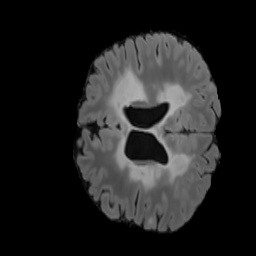
\includegraphics[width=.32\textwidth]{images/tr_images/tr175_input.jpg}\hfill
    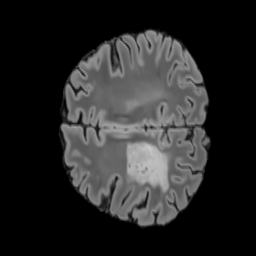
\includegraphics[width=.32\textwidth]{images/tr_images/tr943_input.jpg}\hfill
    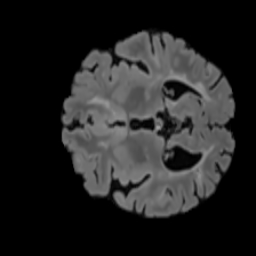
\includegraphics[width=.32\textwidth]{images/tr_images/tr1426_input.jpg}
    %\caption{Image A.}
    %\caption{Image B.}
    %\caption{Image C.}
    \subfigure[tr175]{
\includegraphics[width=.32\textwidth]{images/tr_images/tr175_mask.jpg}\label{fig:tr175}}\hfill
    \subfigure[tr943]{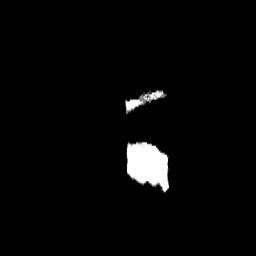
\includegraphics[width=.32\textwidth]{images/tr_images/tr943_mask.jpg}\label{fig:tr943}}\hfill
    \subfigure[tr1426]{
\includegraphics[width=.32\textwidth]{images/tr_images/tr1426_mask.jpg}\label{fig:tr1426}}
    %\caption{Image A.}
    %\caption{Image B.}
    %\caption{Image C.}
\end{figure*}

Sample of images from the validation set: 
\begin{figure*}[!htb]
    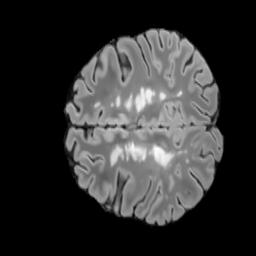
\includegraphics[width=.32\textwidth]{images/ts_images/ts175_input.jpg}\hfill
    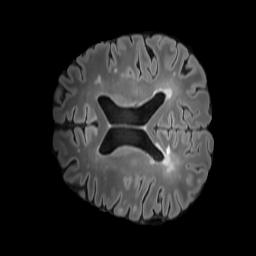
\includegraphics[width=.32\textwidth]{images/ts_images/ts431_input.jpg}\hfill
    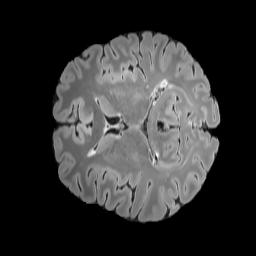
\includegraphics[width=.32\textwidth]{images/ts_images/ts687_input.jpg}
    %\caption{Image A.}
    %\caption{Image B.}
    %\caption{Image C.}
    \subfigure[ts175]{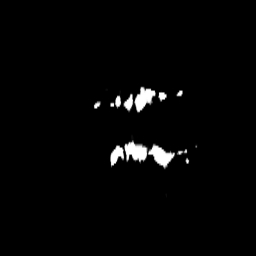
\includegraphics[width=.32\textwidth]{images/ts_images/ts175_mask.jpg}\label{fig:ts175}}\hfill
    \subfigure[ts431]{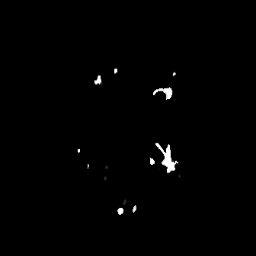
\includegraphics[width=.32\textwidth]{images/ts_images/ts431_mask.jpg}\label{fig:ts431}}\hfill
    \subfigure[ts687]{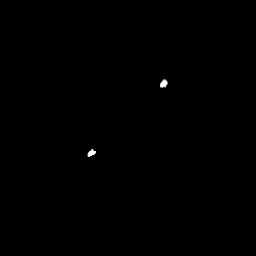
\includegraphics[width=.32\textwidth]{images/ts_images/ts687_mask.jpg}\label{fig:ts687}}
    %\caption{Image A.}
    %\caption{Image B.}
    %\caption{Image C.}
\end{figure*}

\newpage
\section{Evaluation metrics}

% TODO:
The metrics used for evaluation are ...